\documentclass[hanbdout,a4paper,slidestop,dvips,xcolor=pst,blue]{beamer}

\usepackage{beamerthemesplit}
\usepackage[utf8]{inputenc}
\usepackage[spanish]{babel}
\usepackage{graphicx}
\usepackage{pstricks} % PSTricks package
\usepackage{setspace}
\usepackage{multirow}
\usepackage{listings}
\usepackage{pgfpages}
\usepackage{hyperref}
\usepackage{etoolbox}
\usepackage{epstopdf}

\makeatletter
\patchcmd{\beamer@sectionintoc}{\vskip1.5em}{\vskip0.5em}{}{}
\makeatother

\setbeamercovered{dynamic}
\setcounter{tocdepth}{2}
\setbeamercolor{frametitle}{fg=black,bg=white}
\setbeamercolor{section in toc shaded}{fg=black}
\setbeamercolor{section in toc}{fg=red}
\setbeamercolor{subsection in toc shaded}{fg=black}
\setbeamercolor{subsection in toc}{fg=red}
\setbeamerfont{section in toc}{size=\small}
\setbeamerfont{subsection in toc}{size=\small}
\setbeamertemplate{section in toc shaded}[default][99]
\setbeamertemplate{subsection in toc shaded}[default][99]

\AtBeginSection[]
{\begin{frame}[c]
  \frametitle{Índice}
	\tableofcontents[currentsection,
        sectionstyle=show/shaded,
        subsectionstyle=hide]
\end{frame}}

\AtBeginSubsection[]
{\begin{frame}[c]
	\frametitle{Índice}
	\tableofcontents[
  		currentsection,
  		sectionstyle=shaded/shaded,
  		currentsubsection,
  		subsectionstyle=show/shaded/hide
		]
\end{frame}}

\setbeamercolor{frametitle}{fg=black,bg=white}

\setbeamertemplate{frametitle}{
	\begin{centering}
		\insertframetitle
		\par
	\end{centering}
}

\usetheme[secheader]{Boadilla} 

\title[Gestión de la Configuración]{Gestión Avanzada de la \\ Configuración de Sistemas Software}

\author[Pablo S\'{a}nchez]{\alert{Pablo S\'{a}nchez}}

\institute[I2E]{
		   Dpto. Ingenier{\'i}a Inform{\'a}tica y Electr{\'o}nica \\
		   Universidad de Cantabria, Santander (Spain)\\ p.sanchez@unican.es
		   }

\date{}

\begin{document}

\begin{frame}[c]
	\titlepage
	\begin{columns}
		\column{0.50\linewidth}
			\centering
    		
\includegraphics[width=.28\textwidth,keepaspectratio=true]{images/istr.eps}
		\column{0.50\linewidth}
			\centering
			
\includegraphics[width=.25\textwidth,keepaspectratio=true]{images/uc.eps}
	\end{columns}
\end{frame}

\begin{frame}[c]
    \frametitle{\alert{Advertencia}}
    \begin{center}
        Todo el material contenido en este documento  no constituye en modo alguno una obra de referencia o apuntes oficiales mediante los cuales se puedan preparar de manera autónoma las pruebas necesarias para superar la asignatura. \ \\
        \ \\
        Este documento contiene exclusivamente una serie de diapositivas cuyo objetivo es servir de complemento visual a las actividades realizadas en el aula.  \ \\
        \ \\
        Dicho de forma más clara, \alert{estas transparencias no son apuntes y su objetivo no es en modo alguno servir para que el alumno pueda preparar la asignatura.}
    \end{center}
\end{frame}

\begin{frame}[c]
    \frametitle{Objetivos del Tema}
    \begin{enumerate}[<+->]
         \item Recordar y comprender la importancia y objetivos de la gestión de la configuración de sistemas sw.
         \item Comprender los conceptos de \emph{integración} y \emph{entrega continua}.
         \item Comprender el concepto de \emph{DevOps}.
         \item Ser capaz de crear y fusionar ramas utilizando \alert{Git}.
         \item Ser capaz de entender el concepto de flujo de trabajo en gestión de la configuración.
    \end{enumerate}
\end{frame}

\begin{frame}[c]
    \frametitle{Bibliografía}
    \begin{thebibliography}{1}
    \bibitem{}
    Ian Sommerville.
    \newblock {\em {Software Engineering}}.
    \newblock Addison Wesley, 9 edition, April 2010.

    \bibitem{}
    Scott Chacon.
    \newblock {\em {Pro Git}}.
    \newblock Apress, 2 edition 2014.

\end{thebibliography}
\end{frame}

\section{Introducción}

\subsection[Ciclo de Vida Sw]{Ciclo de Vida Software}

%%% Introducción, Contextualización del tema
\begin{frame}[t]
	\frametitle{Gestión de la Configuración de Sistemas Software}
	\ \\
	\only<1|handout:0>{
	\rput[lt](0,1){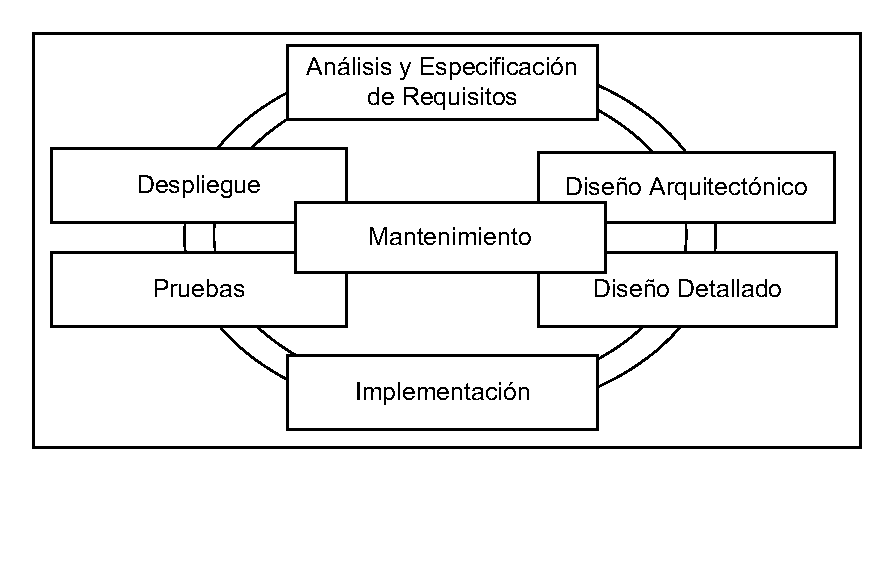
\includegraphics[clip=true,width=\linewidth]{images/introduction/swProcess00.eps}}}
	\only<2>{
	\rput[lt](0,1){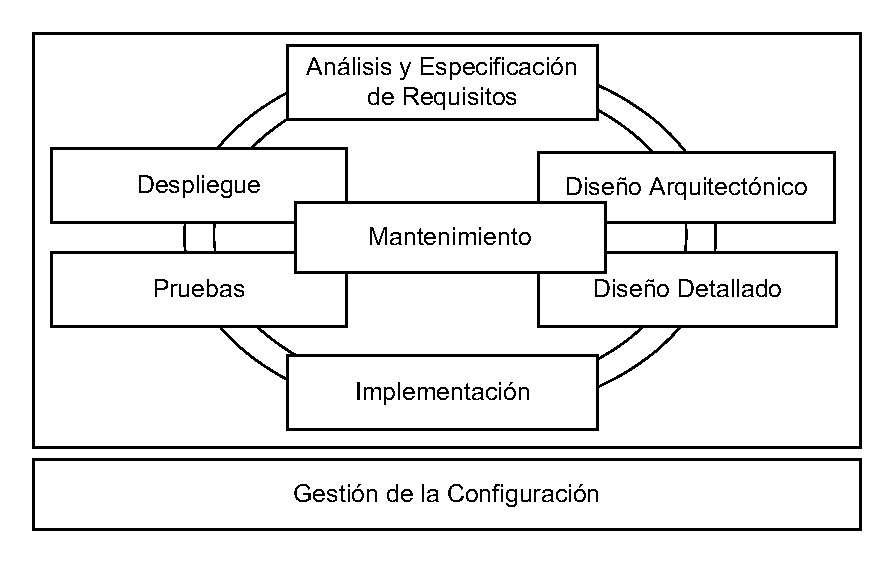
\includegraphics[clip=true,width=\linewidth]{images/introduction/swProcess01.eps}}}
\end{frame}

\subsection[Motivación y Objetivos]{Motivación y Objetivos}

\begin{frame}[c]
	\frametitle{¿Por Qué Necesitamos la Gestión de la Configuración?}
	\begin{enumerate}
		\item<1-> ¿Qué he cambiado? ¿Cómo hago si no hubiese pasado nada?
		\item<2-> Problema de la copia correcta.
		\item<3-> Desarrollo distribuido de software.
		\item<4-> Problema de que \emph{Google} encuentra los archivos mejor que yo.
	\end{enumerate}
\end{frame}

\begin{frame}
	\frametitle{Situación a evitar}
	\begin{center}
		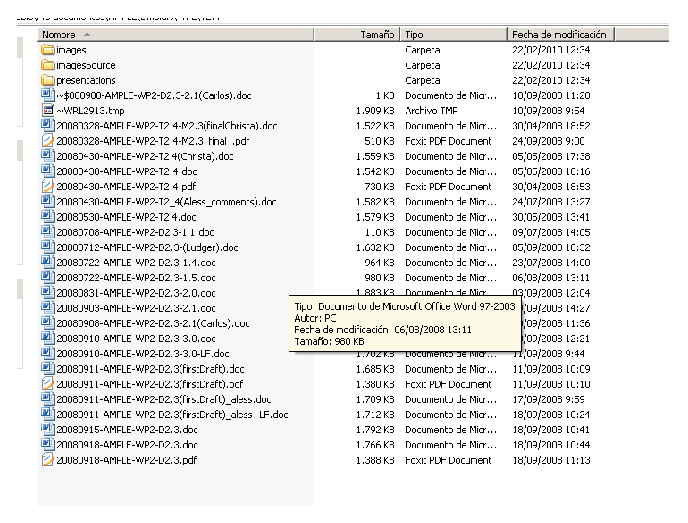
\includegraphics[width=.8\linewidth,keepaspectratio=true]{images/introduction/ampleFolder.eps}
	\end{center}
\end{frame}

\section{Terminología Básica}

\begin{frame}[c]
	\frametitle{Definiciones}
	   \begin{block}{Configuration Item}
		  Artefacto o conjunto de artefactos susceptible de poseer varias versiones.
	   \end{block}
	\uncover<2->{
	   \begin{block}{Version}
		    Instancia de un ítem de configuración que difiere de alguna
            manera de otras instancias del mismo artefacto.
	   \end{block}
    }
	\uncover<3->{
        \begin{block}{Release}
		  Versión de un item de configuración (puede ser un sistema entero) que se distribuye a los clientes.
	   \end{block}
    }
\end{frame}

\begin{frame}
	\frametitle{Definiciones}
	\begin{block}{Baseline}
		Conjunto de versiones concretas de los diferentes items de configuración, que constituyen un estado significativo,
        claramente identificado, controlado y aprobado en la evolución de un producto.
	\end{block}
\end{frame}

\section{Procesos de Gestión de la Configuración Sw}

\subsection{Gestión de la Configuración Sw}

\begin{frame}[t]
	\frametitle{Áreas de la Gestión de la Configuración Sw}
    \only<1|handout:0>{
    \rput[lt](0.5,0){
        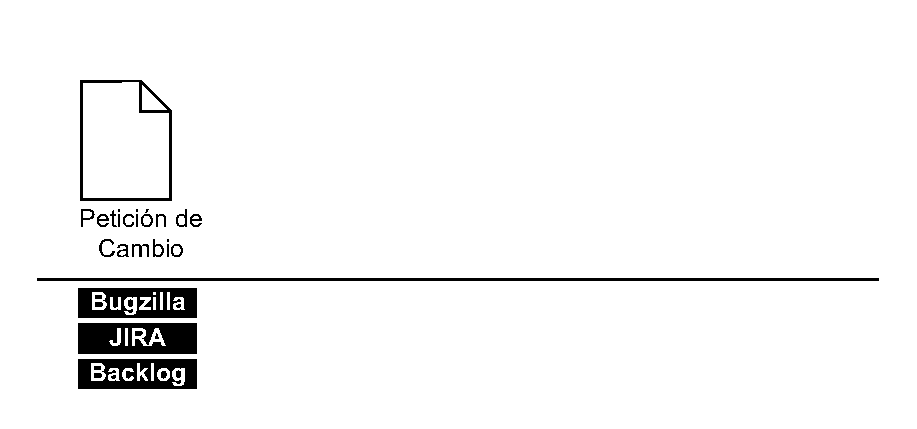
\includegraphics[width=11cm,keepaspectratio=true]{images/elementosGc/esquemaGc00.eps}}}
    \only<2|handout:0>{
    \rput[lt](0.5,0){
        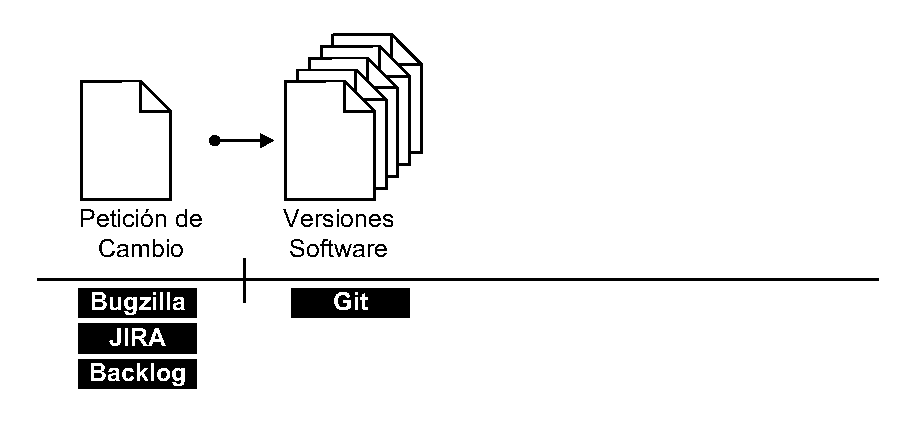
\includegraphics[width=11cm,keepaspectratio=true]{images/elementosGc/esquemaGc01.eps}}}
    \only<3|handout:0>{
    \rput[lt](0.5,0){
        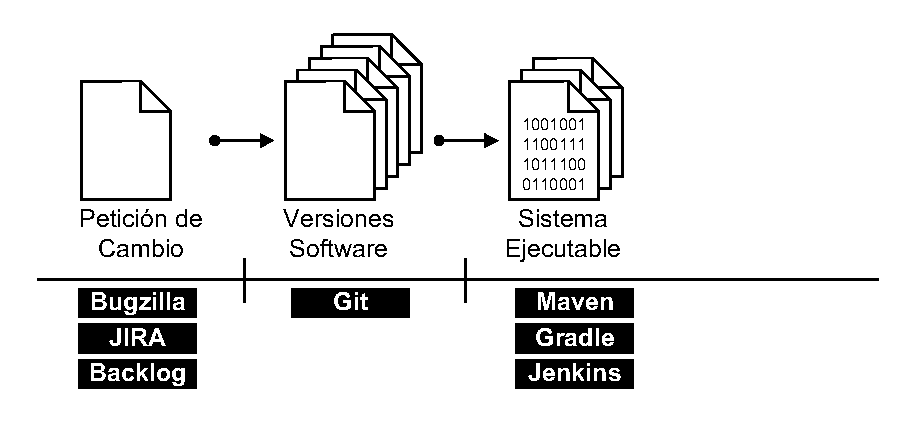
\includegraphics[width=11cm,keepaspectratio=true]{images/elementosGc/esquemaGc02.eps}}}
    \only<4>{
    \rput[lt](0.5,0){
        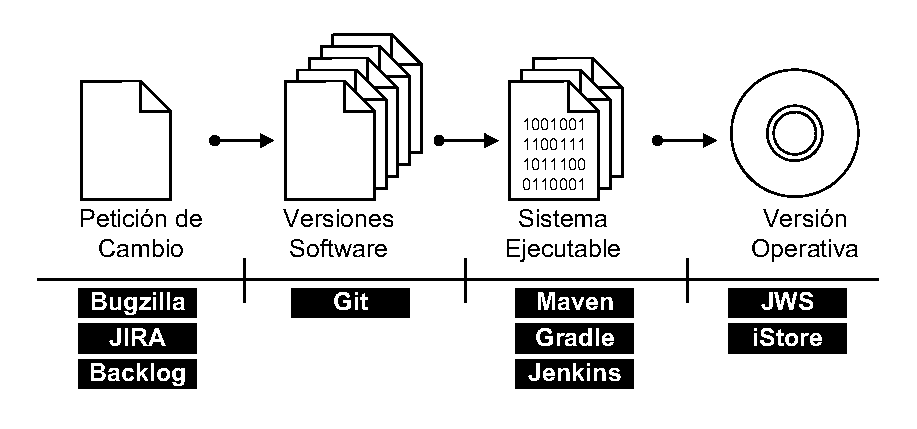
\includegraphics[width=11cm,keepaspectratio=true]{images/elementosGc/esquemaGc03.eps}}}
\end{frame}

\subsection{Integración y Entrega Continua}

\begin{frame}[t]
	\frametitle{Integración y Entrega Continua}
    \only<1|handout:0>{
    \rput[lt](0.5,0){
        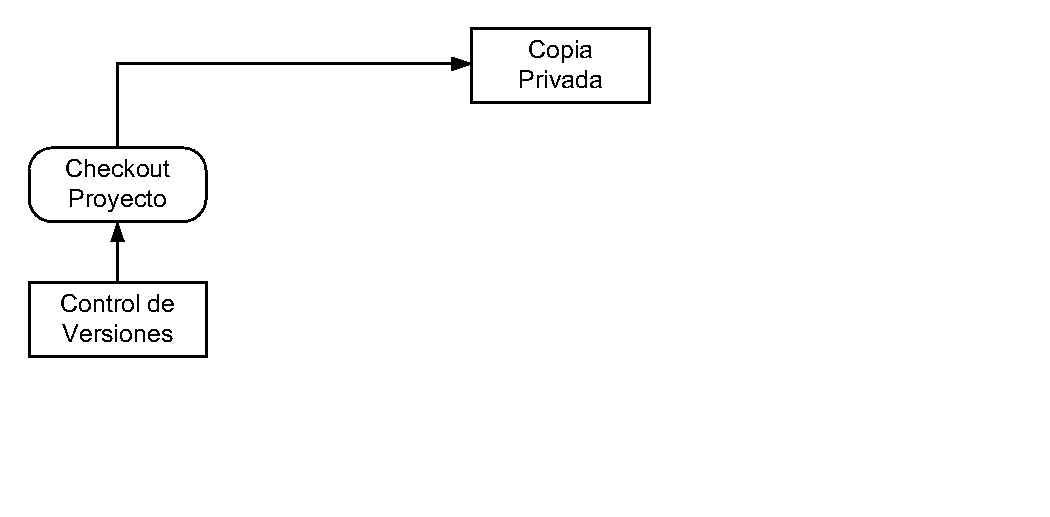
\includegraphics[width=11cm,keepaspectratio=true]{images/elementosGc/ci00.eps}}}
    \only<2|handout:0>{
    \rput[lt](0.5,0){
        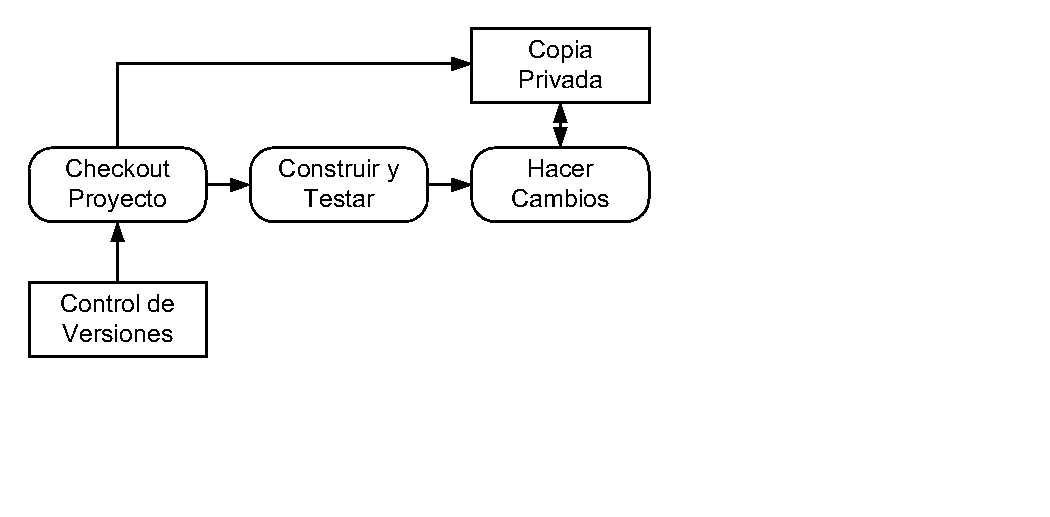
\includegraphics[width=11cm,keepaspectratio=true]{images/elementosGc/ci01.eps}}}
    \only<3|handout:0>{
    \rput[lt](0.5,0){
        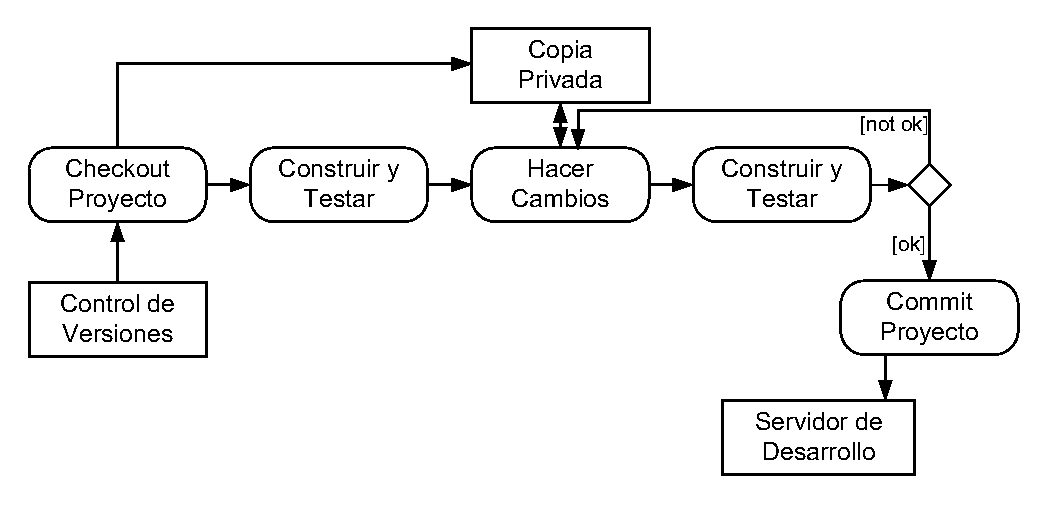
\includegraphics[width=11cm,keepaspectratio=true]{images/elementosGc/ci02.eps}}}
    \only<4|handout:0>{
    \rput[lt](0.5,0){
        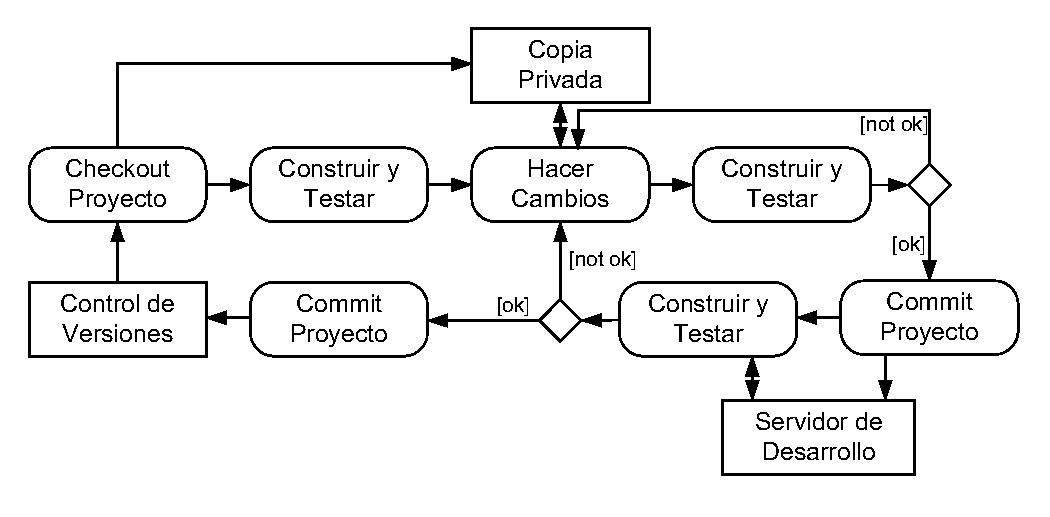
\includegraphics[width=11cm,keepaspectratio=true]{images/elementosGc/ci03.eps}}}
    \only<5>{
    \rput[lt](0.5,0){
        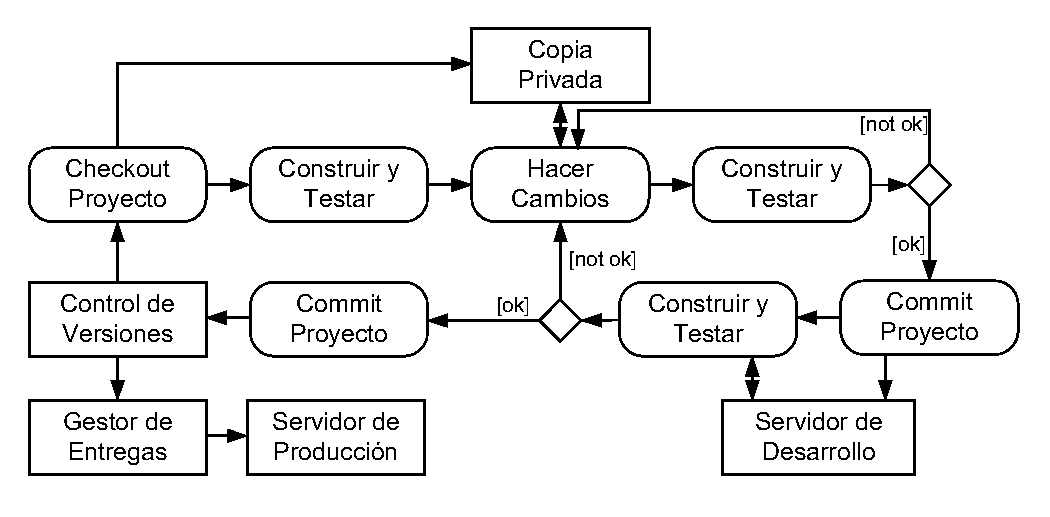
\includegraphics[width=11cm,keepaspectratio=true]{images/elementosGc/ci04.eps}}}
\end{frame}

% \subsection{Entrega Continua}

%\begin{frame}[c]
%	\frametitle{Integración Continua}
%	\begin{enumerate}[<+->]
%		\item Todos los desarrolladores hacen integraciones frecuentes.
%        \item Cada integración se testea automáticamente.
%        \item Los errores descubiertos por los tests se solucionan tan pronto como sea posible.
%        \item Todos los desarrolladores trabajan sobre versiones del sistema lo más actualizadas posibles.
%	\end{enumerate}
%\end{frame}
%
%\begin{frame}[c]
%	\frametitle{Entrega Continua}
%	\begin{enumerate}[<+->]
%	   \item El sw bajo desarrollo se va entregando a lo largo de su ciclo de vida.
%       \item Es prioridad mantener el sw entregrable que trabajar en nuevas funcionalidades.
%       \item Se debe ser capaz de realizar entregas de un producto pulsando un botón.
%    \end{enumerate}
%\end{frame}

\subsection{DevOps}

\begin{frame}[c]
	\frametitle{DevOps}
	\begin{enumerate}[<+->]
	   \item Unión de los equipos de desarrollo (\emph{Development}) y operaciones (\emph{Operations}) con el objetivo de mejorar la calidad del software.
       \item Filosofía \emph{you build it, you run it}.
       \item Técnicas frecuentemente utilizadas:
            \begin{itemize}
                \item Integración y entrega continua.
                \item Automatización de la infraestructura (\emph{platform as code})
                \item Desarrollo basado en microservicios.
                %% Observed requirements es monitorizar las acciones de usuario.
                %% Wish list de Amazon como listas para comparar productos.
                \item Monitorización de operaciones y análisis de datos: \emph{observed requirements}, \emph{AB tests}, \emph{canary test}.
            \end{itemize}
    \end{enumerate}	
\end{frame}

\section{Control de Versiones con Git}

\subsection{Características de Git}

\begin{frame}[c]
	\frametitle{Git}
	 \begin{enumerate}[<+->]
        \item Distribuido y descentralizado.
        \item Instantáneas en lugar de incrementos.
        \item Operaciones preferentemente locales.
        \item Verifica la integridad de los archivos.
	 \end{enumerate}
\end{frame}

\begin{frame}[c]
	\frametitle{Sistema Centralizado}
	 \begin{center}
		\includegraphics[width=0.80\linewidth,keepaspectratio=true]{images/git/centralizado.eps}
	 \end{center}
\end{frame}

\begin{frame}[c]
	\frametitle{Problema Sistemas Centralizados}
	 \begin{center}
		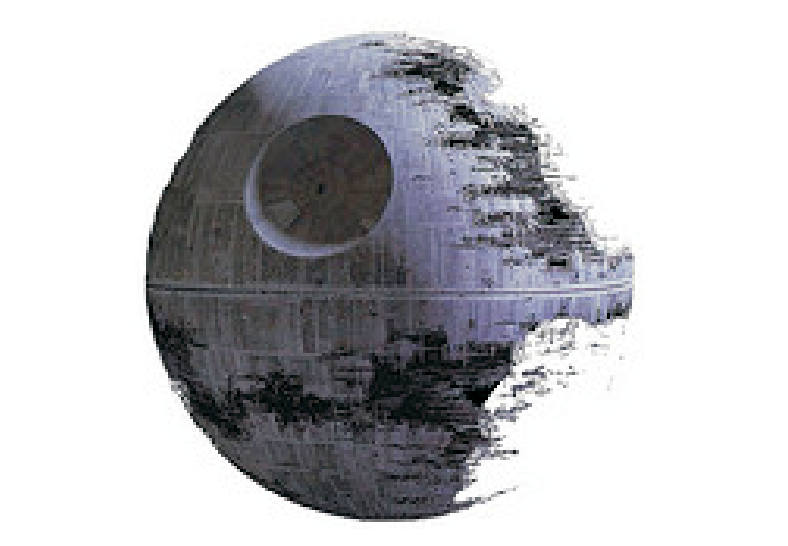
\includegraphics[width=0.80\linewidth,keepaspectratio=true]{images/git/deathStar.eps}
	 \end{center}
\end{frame}

\begin{frame}[c]
	\frametitle{Sistema Distribuido y Descentralizado}
	 \begin{center}
		\includegraphics[width=0.50\linewidth,keepaspectratio=true]{images/git/descentralizado.eps}
	 \end{center}
\end{frame}

\subsection{Acciones Básicas}

\begin{frame}[c]
	\frametitle{Comienzo de un Versionado con Git}
	 \begin{description}[<+->]
        \item[Init] Crea un repositorio en un directorio o proyecto existente.
        \item[Clone] \alert<3->{Clona} un repositorio (remoto) en un directorio concreto.
	 \end{description}
\end{frame}

\begin{frame}[c]
	\frametitle{Estructura de Proyectos en Git}
	 \begin{center}
		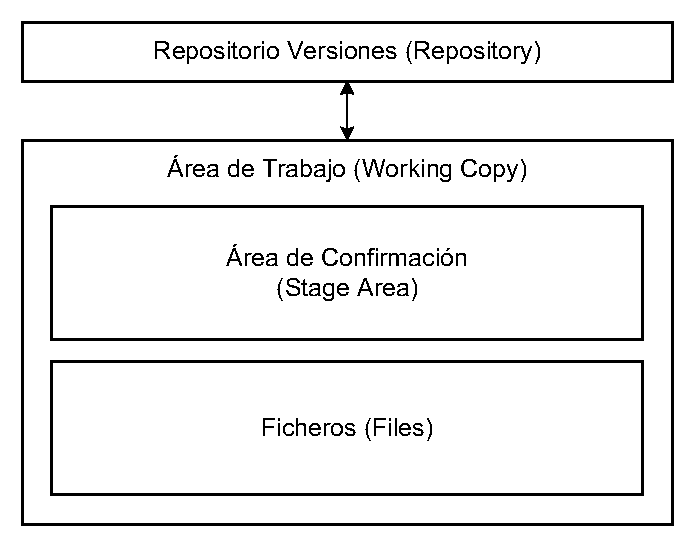
\includegraphics[width=0.75\linewidth,keepaspectratio=true]{images/git/estructuraDirectorios.eps}
	 \end{center}
\end{frame}

\begin{frame}[t]
	\frametitle{Ciclo de Vida de Ficheros en Git}
    \only<1|handout:0>{
    \rput[lt](0,0){
        \includegraphics[width=12cm,keepaspectratio=true]{images/git/cicloDeVida00.eps}}}
    \only<2|handout:0>{
    \rput[lt](0,0){
        \includegraphics[width=12cm,keepaspectratio=true]{images/git/cicloDeVida01.eps}}}
    \only<3|handout:0>{
    \rput[lt](0,0){
        \includegraphics[width=12cm,keepaspectratio=true]{images/git/cicloDeVida02.eps}}}
    \only<4|handout:0>{
    \rput[lt](0,0){
        \includegraphics[width=12cm,keepaspectratio=true]{images/git/cicloDeVida03.eps}}}
    \only<5|handout:0>{
    \rput[lt](0,0){
        \includegraphics[width=12cm,keepaspectratio=true]{images/git/cicloDeVida04.eps}}}
    \only<6|handout:0>{
    \rput[lt](0,0){
        \includegraphics[width=12cm,keepaspectratio=true]{images/git/cicloDeVida05.eps}}}
    \only<7|handout:0>{
    \rput[lt](0,0){
        \includegraphics[width=12cm,keepaspectratio=true]{images/git/cicloDeVida06.eps}}}
    \only<8>{
    \rput[lt](0,0){
        \includegraphics[width=12cm,keepaspectratio=true]{images/git/cicloDeVida07.eps}}}
\end{frame}

\begin{frame}[c]
	\frametitle{Comandos Básicos}
	 \begin{description}[<+->]
        \item[status] Muestra el estado del directorio de trabajo.
%%        \item[.gitignore] Fichero que contiene una lista de archivos que deben ser ignorados por el control de versiones.
        \item[log] Muestra el historial de \emph{commits} realizados.
	 \end{description}
\end{frame}

\subsection{Esquema de Versionado}

\begin{frame}[c]
	\frametitle{Versionado basado en Deltas}
	 \begin{center}
		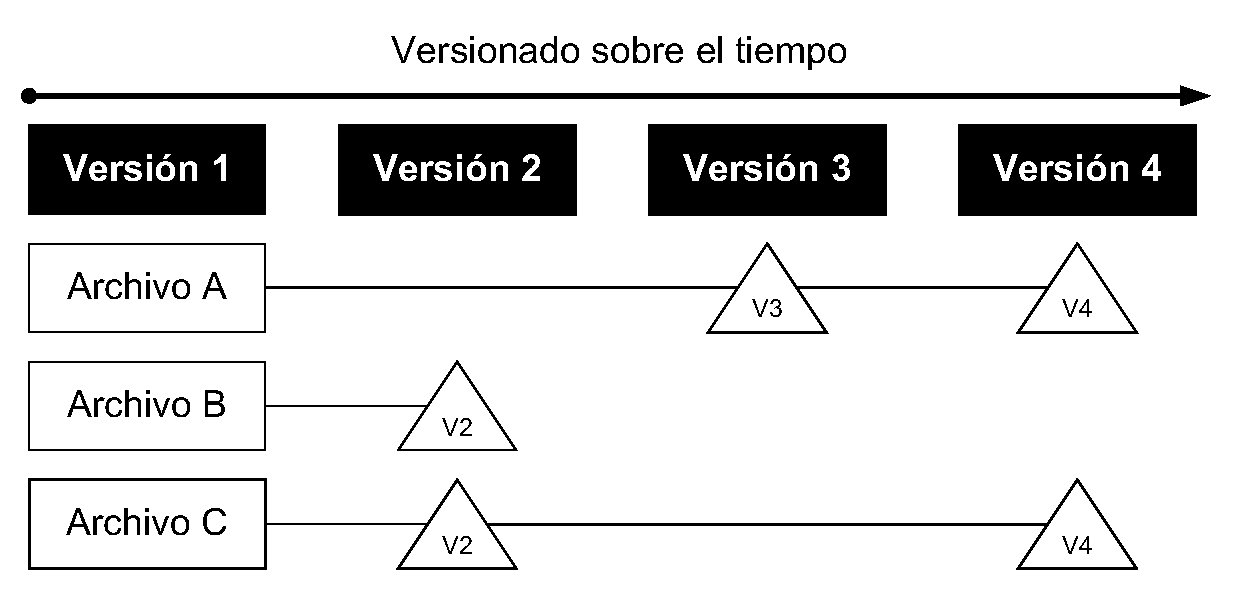
\includegraphics[width=\linewidth,keepaspectratio=true]{images/git/deltas.eps}
	 \end{center}
\end{frame}

\begin{frame}[c]
	\frametitle{Versionado basado en Instantáneas}
	 \begin{center}
		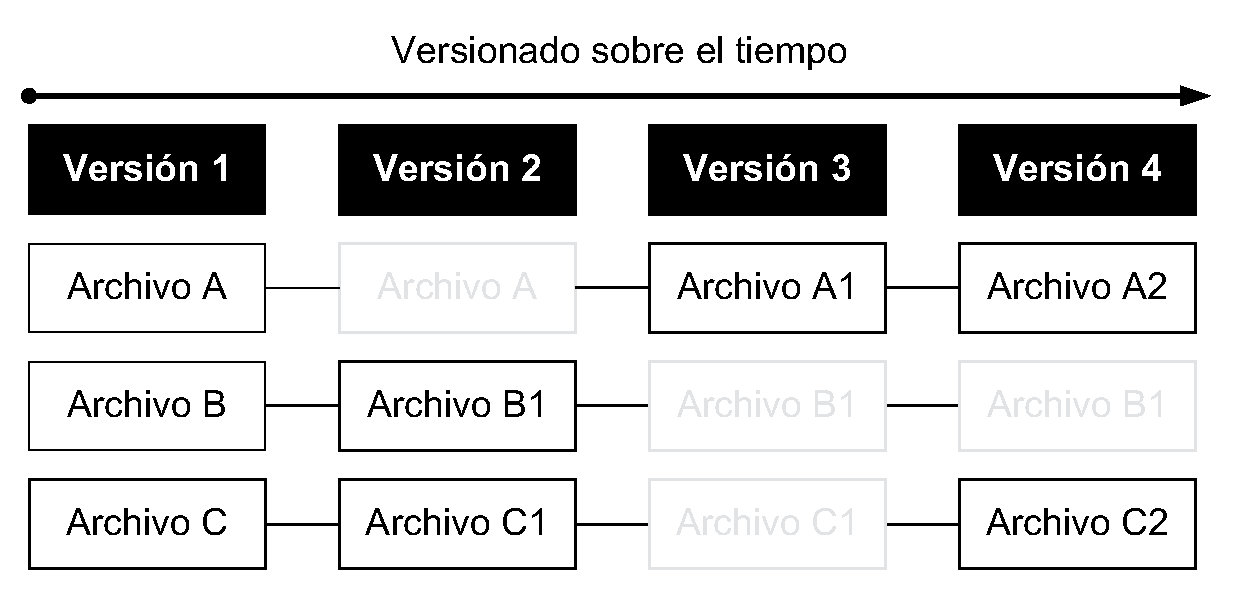
\includegraphics[width=\linewidth,keepaspectratio=true]{images/git/snapshots.eps}
	 \end{center}
\end{frame}

\begin{frame}[t]
	\frametitle{Estructura de Versionado en Git}
    \only<1|handout:0>{
    \rput[lt](2.5,-0.5){
        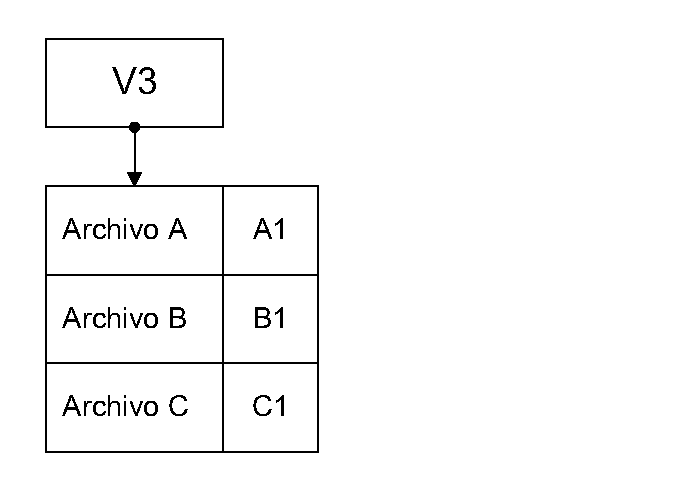
\includegraphics[width=7cm,keepaspectratio=true]{images/git/commitStructure00.eps}}}
    \only<2>{
    \rput[lt](2.5,-0.5){
        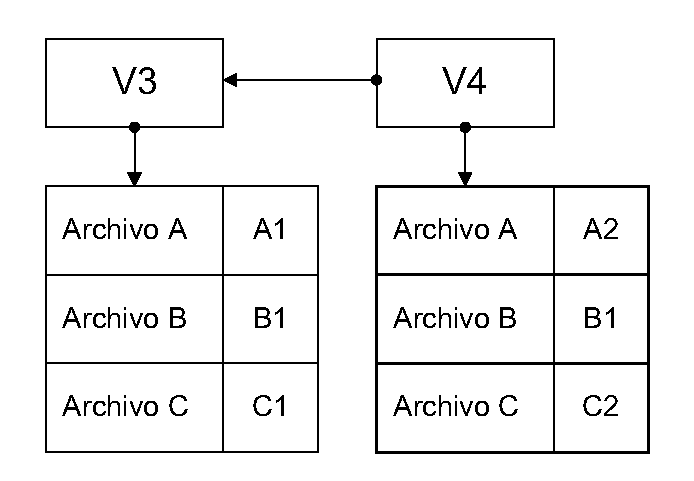
\includegraphics[width=7cm,keepaspectratio=true]{images/git/commitStructure01.eps}}}
\end{frame}

\subsection{Ramificación y Fusión}

\begin{frame}
	\frametitle{Ramificación y Fusión}
    \only<1|handout:0>{
    \rput[lt](0.5,-1.5){
        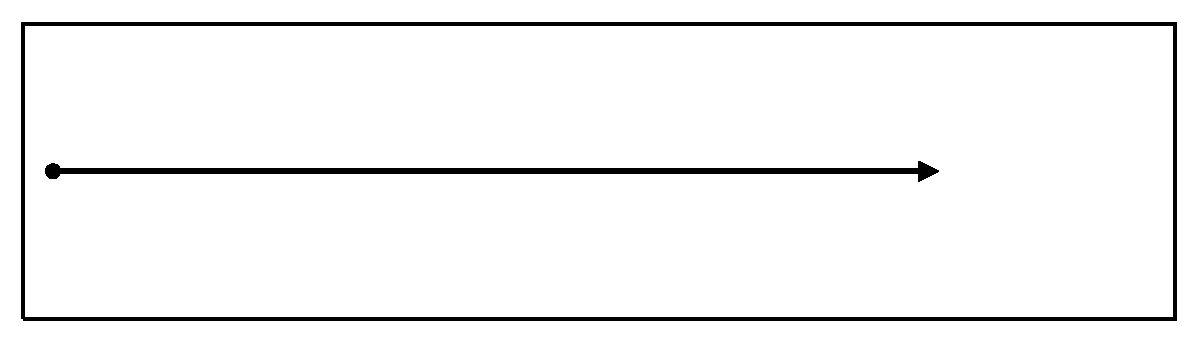
\includegraphics[width=11cm,keepaspectratio=true]{images/git/branching00.eps}}}
    \only<2|handout:0>{
    \rput[lt](0.5,-1.5){
        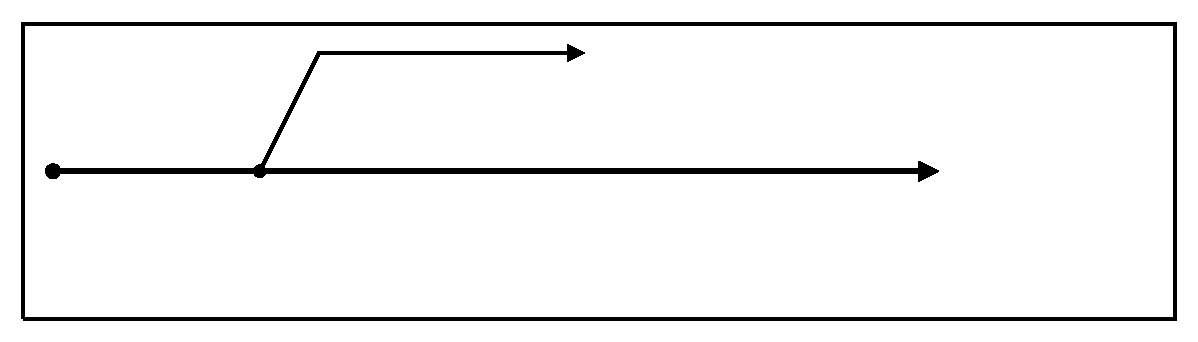
\includegraphics[width=11cm,keepaspectratio=true]{images/git/branching01.eps}}}
    \only<3|handout:0>{
    \rput[lt](0.5,-1.5){
        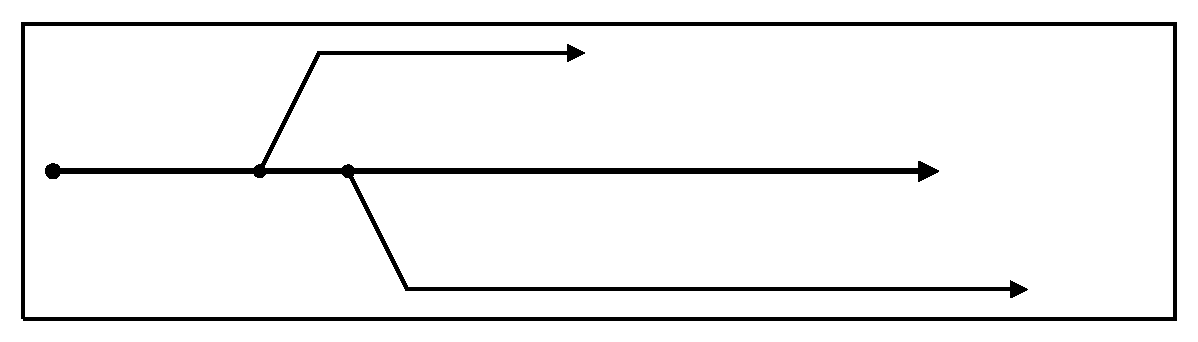
\includegraphics[width=11cm,keepaspectratio=true]{images/git/branching02.eps}}}
    \only<4|handout:0>{
    \rput[lt](0.5,-1.5){
        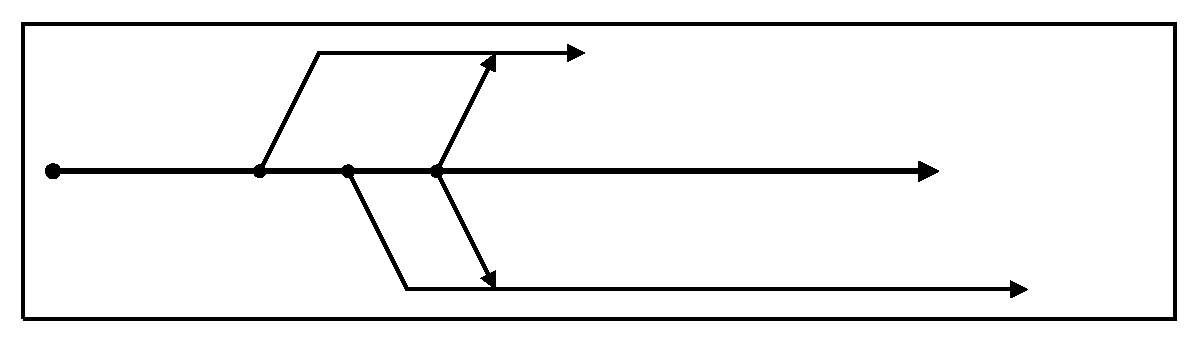
\includegraphics[width=11cm,keepaspectratio=true]{images/git/branching03.eps}}}
    \only<5>{
    \rput[lt](0.5,-1.5){
        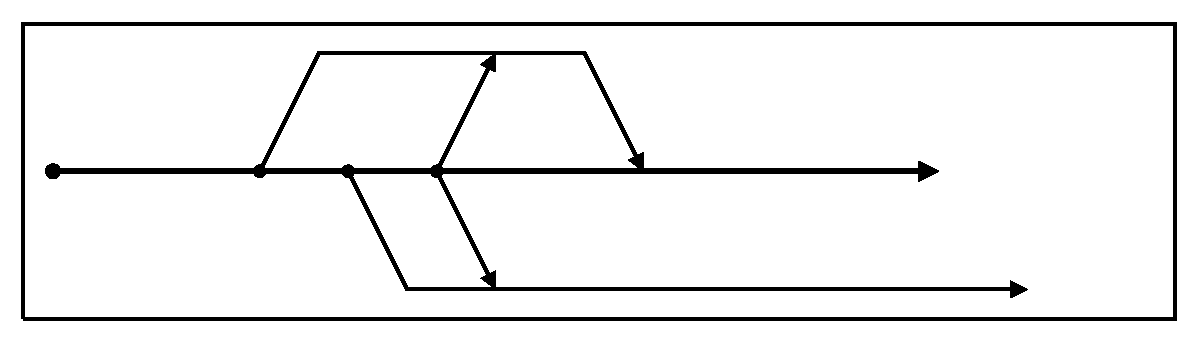
\includegraphics[width=11cm,keepaspectratio=true]{images/git/branching04.eps}}
    }
\end{frame}

\begin{frame}[t]
	\frametitle{Ramificación}
    \only<1|handout:0>{
    \rput[lt](1,0){
        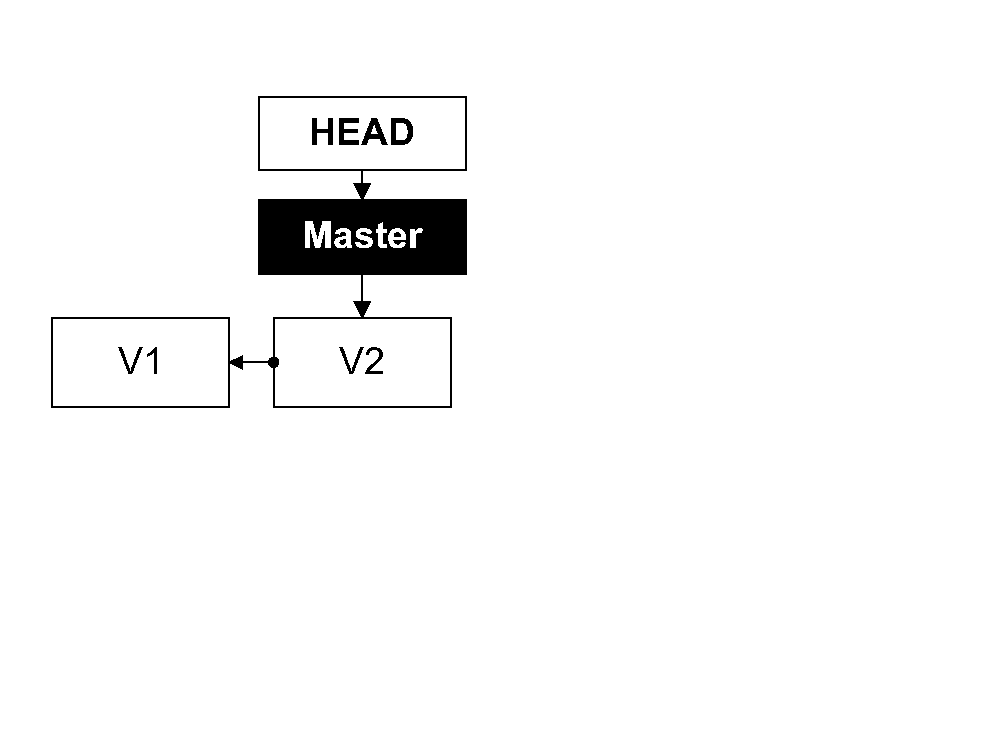
\includegraphics[width=9cm,keepaspectratio=true]{images/git/crearRama00.eps}}}
    \only<2|handout:0>{
    \rput[lt](1,0){
        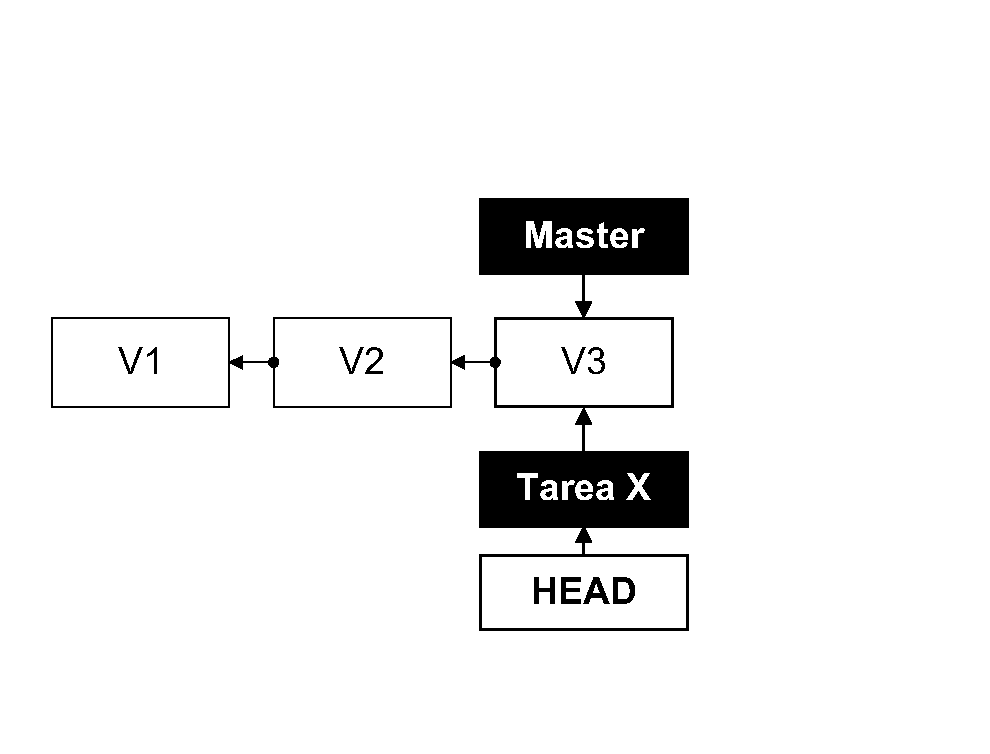
\includegraphics[width=9cm,keepaspectratio=true]{images/git/crearRama01.eps}}}
    \only<3|handout:0>{
    \rput[lt](1,0){
        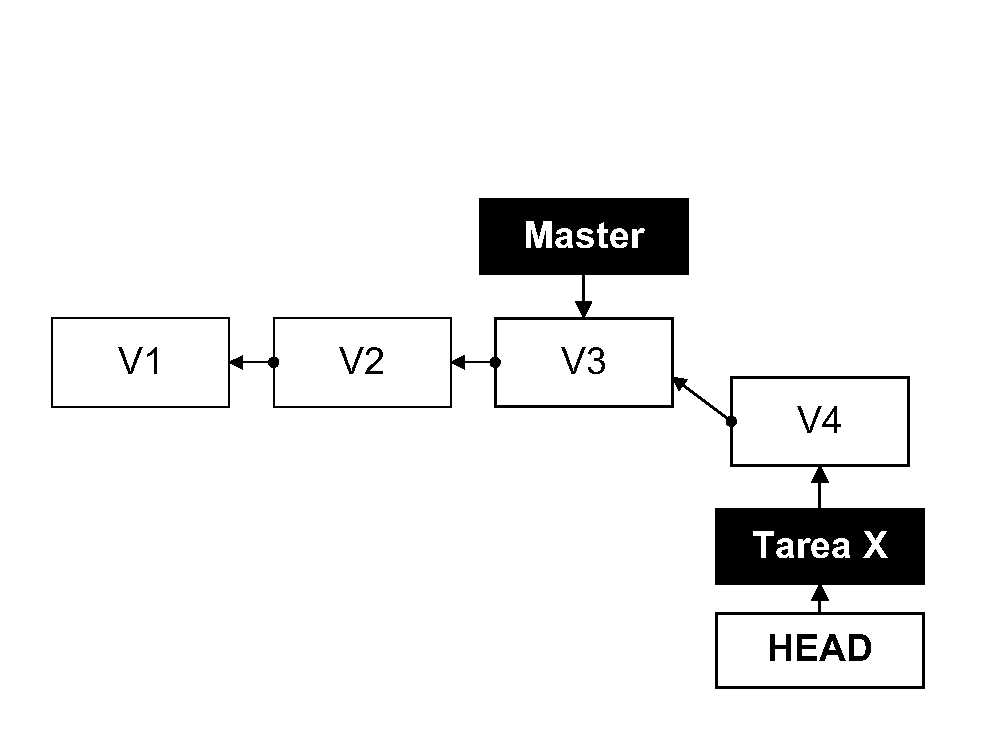
\includegraphics[width=9cm,keepaspectratio=true]{images/git/crearRama02.eps}}}
    \only<4|handout:0>{
    \rput[lt](1,0){
        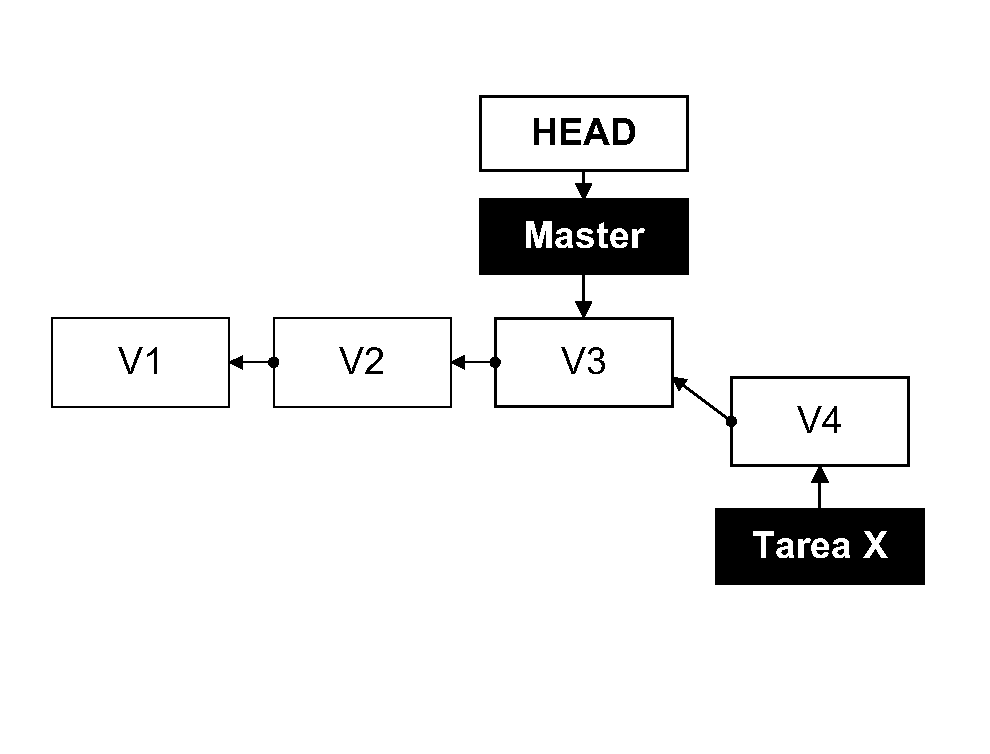
\includegraphics[width=9cm,keepaspectratio=true]{images/git/crearRama03.eps}}}
    \only<5|handout:0>{
    \rput[lt](1,0){
        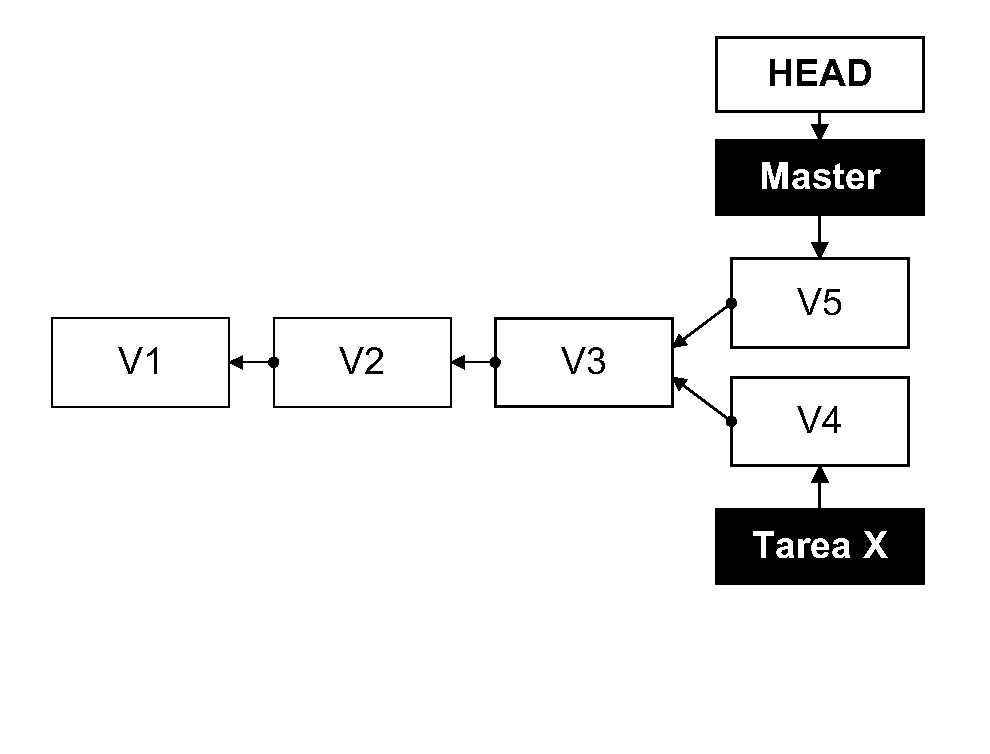
\includegraphics[width=9cm,keepaspectratio=true]{images/git/crearRama04.eps}}}
    \only<6>{
    \rput[lt](1,0){
        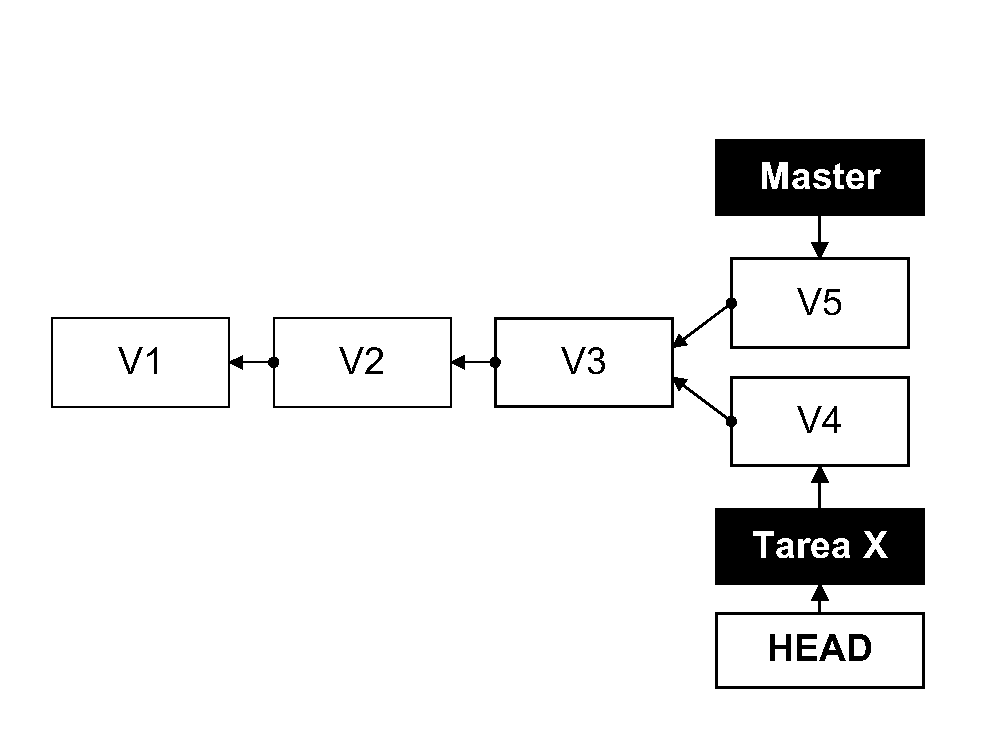
\includegraphics[width=9cm,keepaspectratio=true]{images/git/crearRama05.eps}}}
\end{frame}

\begin{frame}[t]
	\frametitle{Fusión por Avance Rápido}
    \only<1>{
    \rput[lt](0.5,-0.5){
        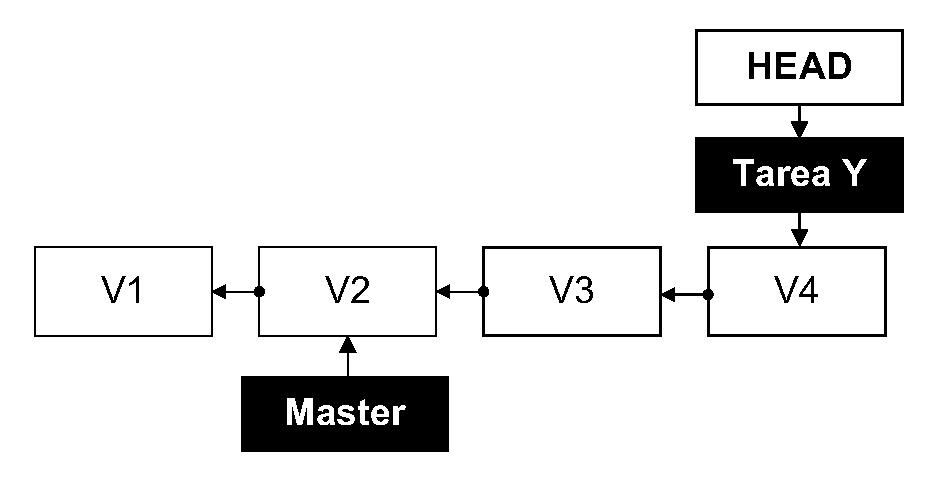
\includegraphics[width=10cm,keepaspectratio=true]{images/git/fastForward00.eps}}}
    \only<2>{
    \rput[lt](0.5,-0.5){
        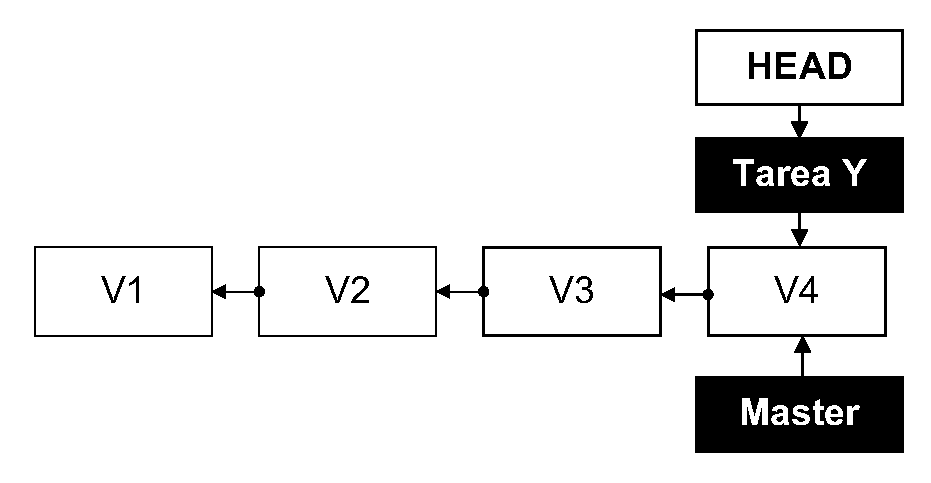
\includegraphics[width=10cm,keepaspectratio=true]{images/git/fastForward01.eps}}}
\end{frame}

\begin{frame}[t]
	\frametitle{Fusión por Recursión}
    \only<1|handout:0>{
    \rput[lt](0.5,-0.5){
        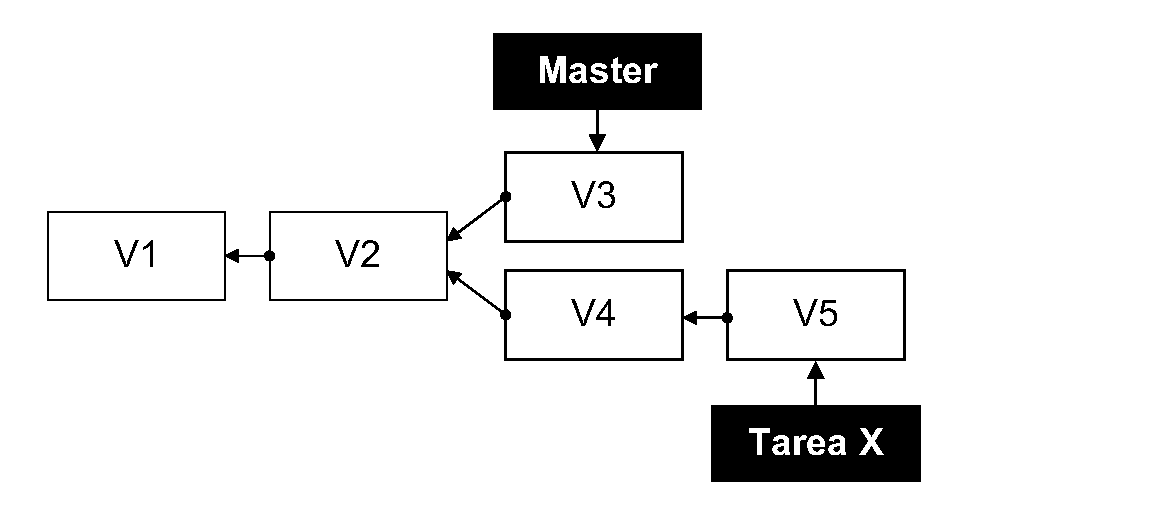
\includegraphics[width=10cm,keepaspectratio=true]{images/git/recursion00.eps}}}
    \only<2>{
    \rput[lt](0.5,-0.5){
        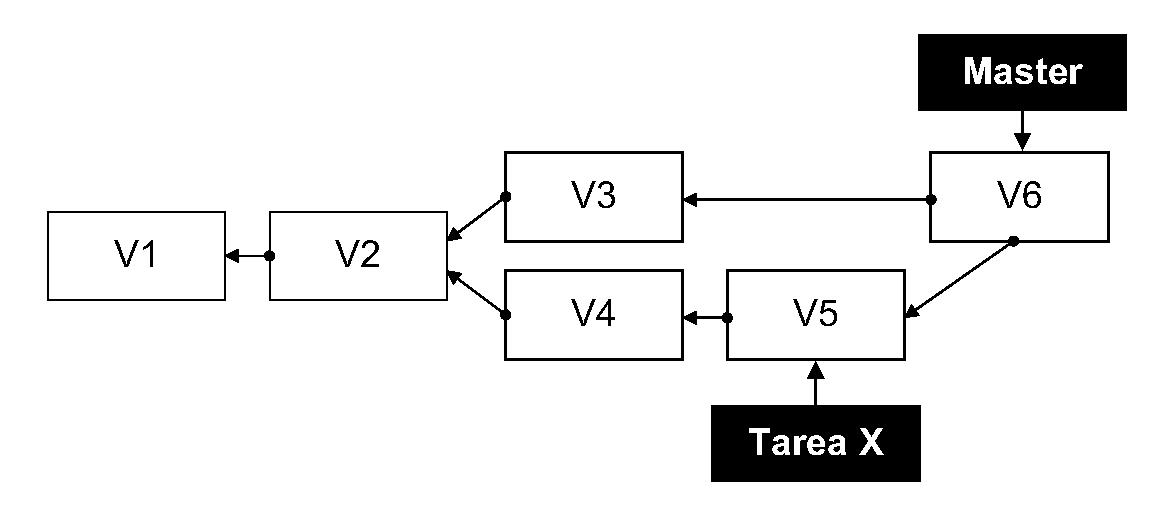
\includegraphics[width=10cm,keepaspectratio=true]{images/git/recursion01.eps}}}
\end{frame}

\begin{frame}[c]
    \frametitle{Resolución de Conflictos}
    \begin{enumerate}[<+->]
        \item Los cambios no conflictivos (diferentes partes de un mismo archivo) simplemente se fusionan.
        \item Los cambios conflictivos se marcan y deben resolverse manualmente.
    \end{enumerate}
\end{frame}

\begin{frame}[t]
	\frametitle{Fusión por Reorganización}
    \only<1|handout:0>{
    \rput[lt](0.5,-0.5){
        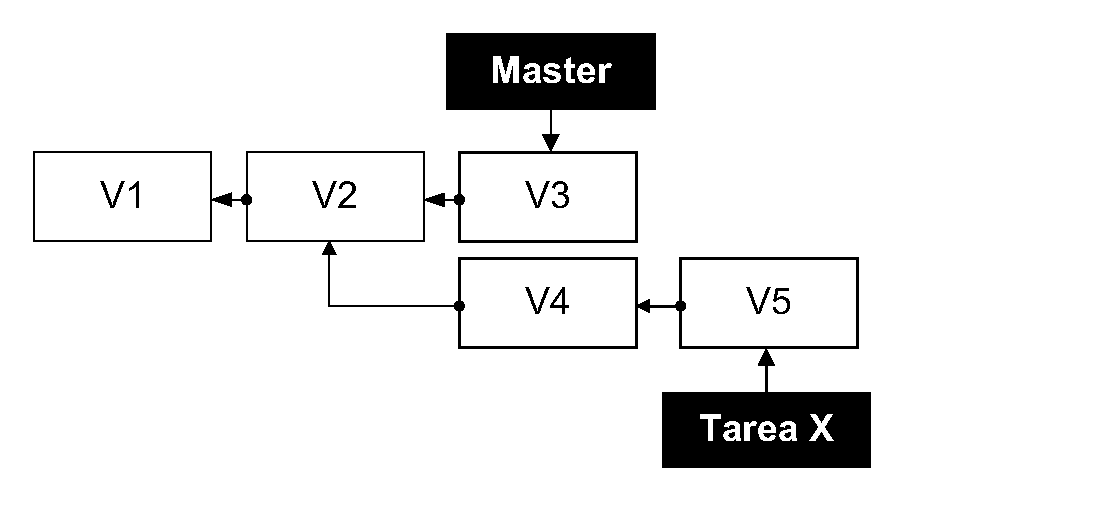
\includegraphics[width=10cm,keepaspectratio=true]{images/git/rebase00.eps}}}
    \only<2>{
    \rput[lt](0.5,-0.5){
        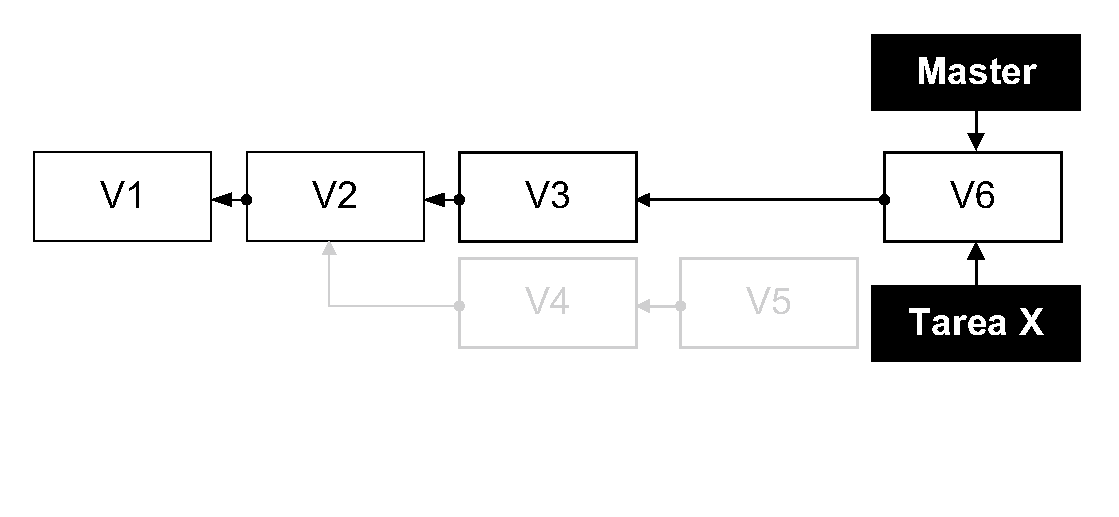
\includegraphics[width=10cm,keepaspectratio=true]{images/git/rebase01.eps}}}
\end{frame}

\begin{frame}[c]
	\frametitle{Comandos Ramificación y Fusión}
	 \begin{description}[<+->]
        \item[Branch] Permite la gestión de ramas.
        \item[Checkout] Se desplaza la versión indicada.
        \item[Tag] Asocia una etiqueta a una determinada version para facilitar su identificación.
        \item[Merge] Fusiona dos ramas.
        \item[Rebase] Reorganiza dos ramas.
	 \end{description}
\end{frame}

\subsection{Stashing}

\begin{frame}[c]
	\frametitle{Recogida y Clareado}
	 \begin{description}[<+->]
        \item[stash] Apila el contenido del directorio del trabajo y lo deja como tras el último \emph{commit}.
        \item[stash apply] Restaura un \emph{stash} determinado.
        \item[stash drop] Elimina un \emph{stash} determinado.
        \item[stash pop] Restaura un \emph{stash} y lo borra.
	 \end{description}
\end{frame}

\subsection{Repositorios Remotos}

\begin{frame}[t]
	\frametitle{Clonado y Seguimiento de Ramas}
    \only<1|handout:0>{
    \rput[lt](0,-0.5){
        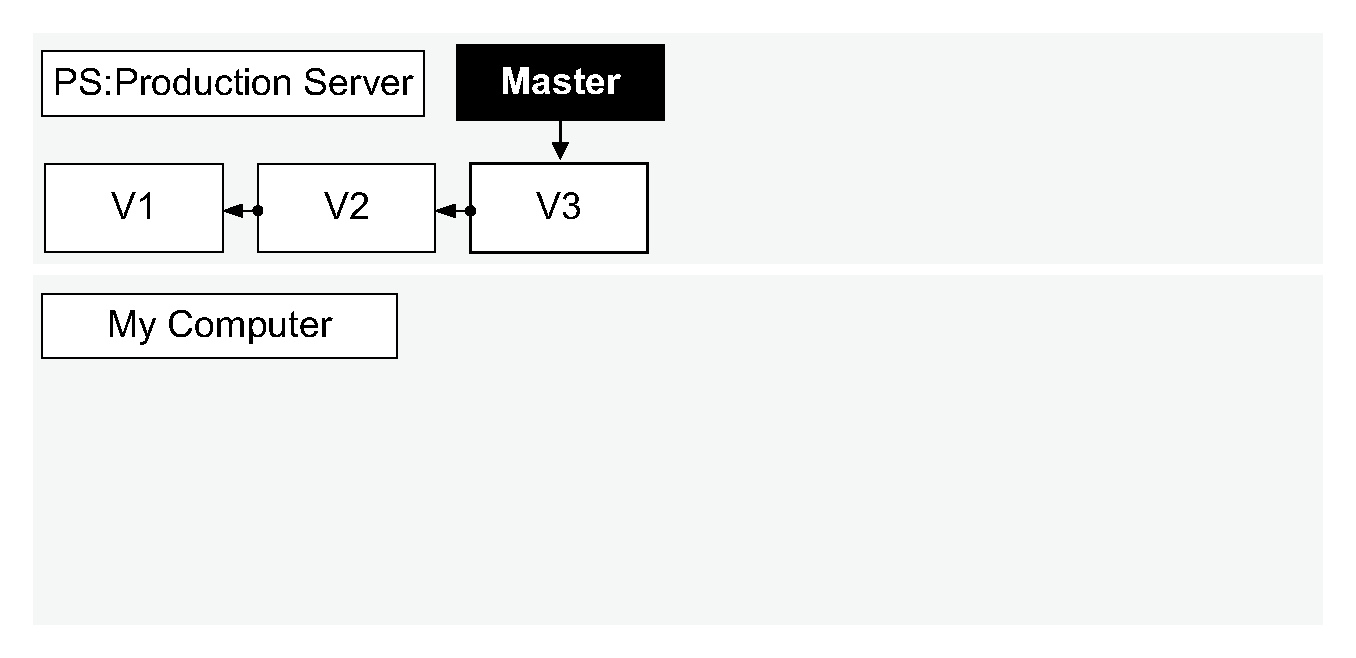
\includegraphics[width=11cm,keepaspectratio=true]{images/git/clone00.eps}}}
    \only<2>{
    \rput[lt](0,-0.5){
        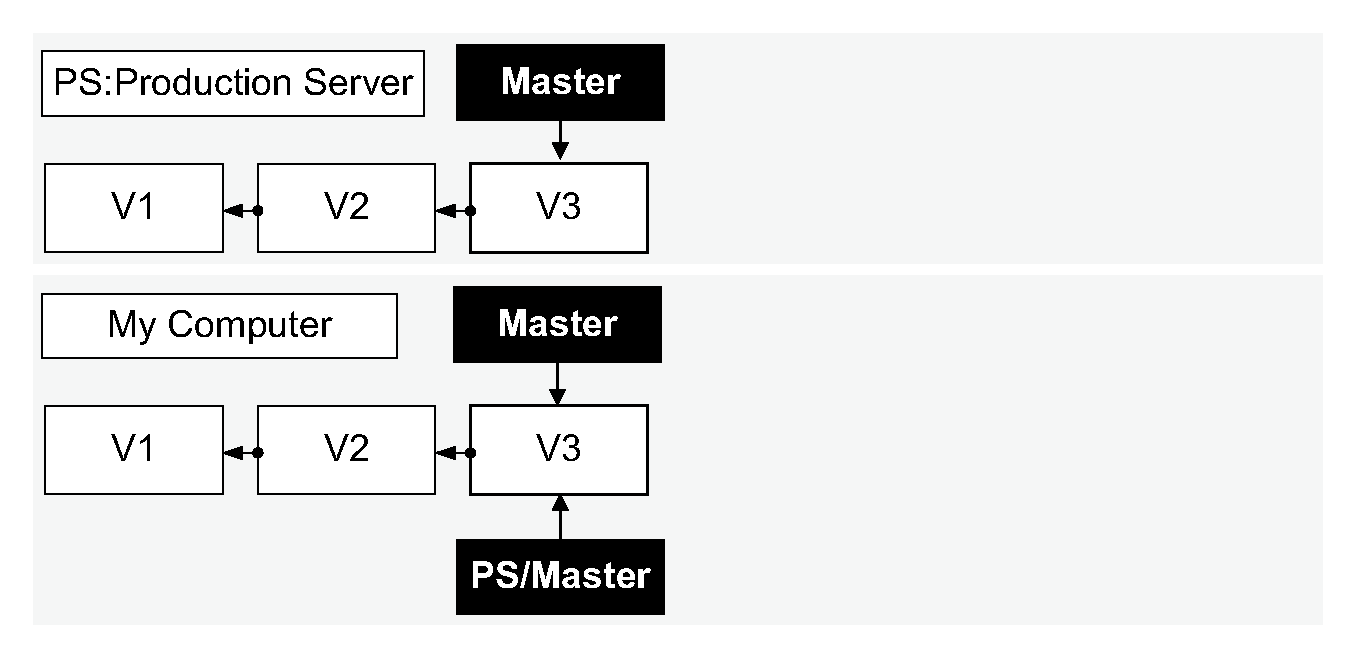
\includegraphics[width=11cm,keepaspectratio=true]{images/git/clone01.eps}}}
\end{frame}

\begin{frame}[t]
	\frametitle{Fetch}
    \only<1|handout:0>{
    \rput[lt](0,-0.5){
        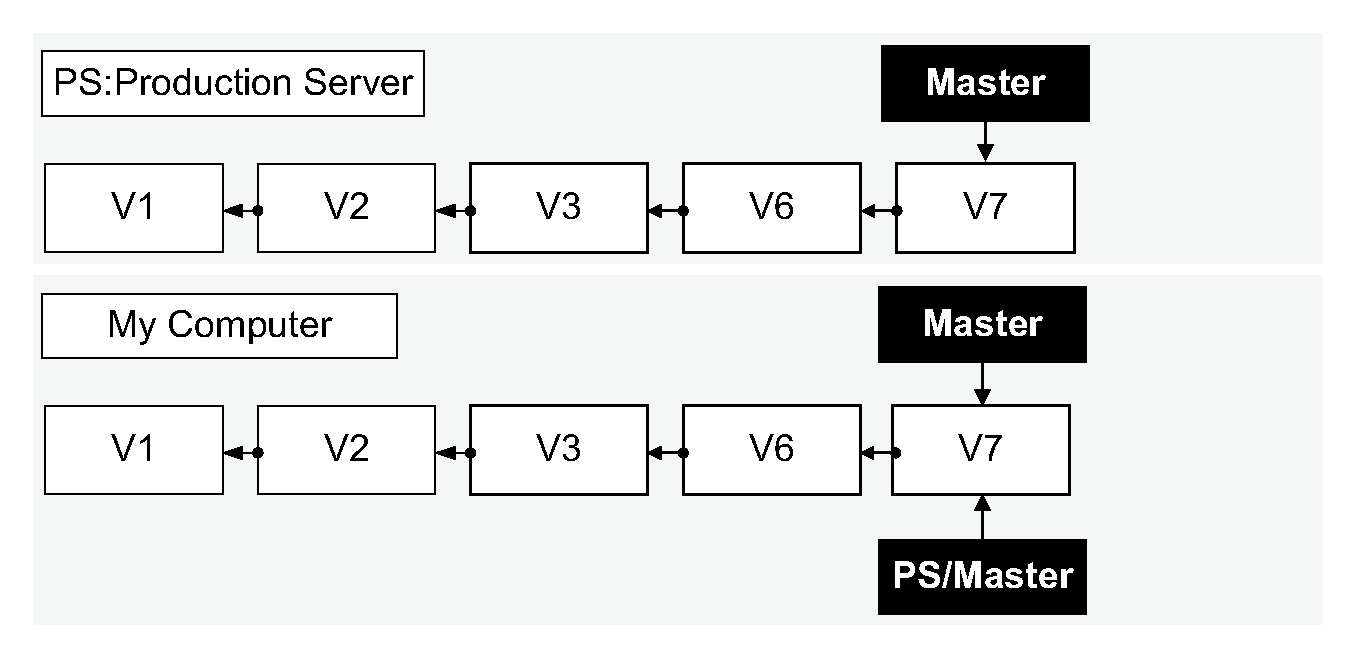
\includegraphics[width=11cm,keepaspectratio=true]{images/git/fetch00.eps}}}
    \only<2>{
    \rput[lt](0,-0.5){
        \includegraphics[width=11cm,keepaspectratio=true]{images/git/fetch01.eps}}}
    \only<3>{
    \rput[lt](0,-0.5){
        \includegraphics[width=11cm,keepaspectratio=true]{images/git/fetch02.eps}}}
\end{frame}

\begin{frame}[t]
	\frametitle{Pull}
    \only<1|handout:0>{
    \rput[lt](0,-0.5){
        \includegraphics[width=11cm,keepaspectratio=true]{images/git/pull00.eps}}}
    \only<2|handout:0>{
    \rput[lt](0,-0.5){
        \includegraphics[width=11cm,keepaspectratio=true]{images/git/pull01.eps}}}
    \only<3>{
    \rput[lt](0,-0.5){
        \includegraphics[width=11cm,keepaspectratio=true]{images/git/pull02.eps}}}
\end{frame}

\begin{frame}[t]
	\frametitle{Push}
    \only<1|handout:0>{
    \rput[lt](0,-0.5){
        \includegraphics[width=11cm,keepaspectratio=true]{images/git/push00.eps}}}
    \only<2|handout:0>{
    \rput[lt](0,-0.5){
        \includegraphics[width=11cm,keepaspectratio=true]{images/git/push01.eps}}}
    \only<3>{
    \rput[lt](0,-0.5){
        \includegraphics[width=11cm,keepaspectratio=true]{images/git/push02.eps}}}
\end{frame}

\begin{frame}[t]
	\frametitle{Conflictos de Sincronización}
    \only<1|handout:0>{
    \rput[lt](2,0){
        \includegraphics[width=8cm,keepaspectratio=true]{images/git/harrySally08.eps}}}
    \only<2|handout:0>{
    \rput[lt](2,0){
        \includegraphics[width=8cm,keepaspectratio=true]{images/git/harrySally09.eps}}}
    \only<3|handout:0>{
    \rput[lt](2,0){
        \includegraphics[width=8cm,keepaspectratio=true]{images/git/harrySally10.eps}}}
    \only<4>{
    \rput[lt](2,0){
        \includegraphics[width=8cm,keepaspectratio=true]{images/git/harrySally11.eps}}}
\end{frame}

\begin{frame}[t]
	\frametitle{Conflictos de Sincronización}
    \only<1|handout:0>{
    \rput[lt](2,0){
        \includegraphics[width=8cm,keepaspectratio=true]{images/git/harrySally12.eps}}}
    \only<2|handout:0>{
    \rput[lt](2,0){
        \includegraphics[width=8cm,keepaspectratio=true]{images/git/harrySally13.eps}}}
    \only<3|handout:0>{
    \rput[lt](2,0){
        \includegraphics[width=8cm,keepaspectratio=true]{images/git/harrySally14.eps}}}
    \only<4|handout:0>{
    \rput[lt](2,0){
        \includegraphics[width=8cm,keepaspectratio=true]{images/git/harrySally15.eps}}}
\end{frame}

\subsection{Deshacer Cambios en Git}

\begin{frame}[c]
	\frametitle{Recuperación de Versiones Antiguas}
	 \begin{description}[<+->]
        \item[reset] Retrocede hasta la versión indicada, borrando los commits intermedios.
        \item[revert] Deshace los cambios realizados hasta volver a la versión indicada. Se crean versiones intermedias para deshacer los cambios.
	 \end{description}
\end{frame}

\begin{frame}[c]
	\frametitle{Borrado y Renombrado}
	 \begin{description}[<+->]
        \item[rm] Borra ficheros (informando al control de versiones).
        \item[mv] Renombra un fichero (informando al control de versiones).
	 \end{description}
\end{frame}

\subsection{Modelos Organizativos con Git}

\begin{frame}[c]
	\frametitle{Centralizado Clásico}
    \begin{center}
        \includegraphics[width=11cm,keepaspectratio=true]{images/git/esquemaCentralizado.eps}
    \end{center}
\end{frame}

\begin{frame}[t]
	\frametitle{Integrador Destacado}
    \only<1|handout:0>{
    \rput[lt](0.5,0){
        \includegraphics[width=11cm,keepaspectratio=true]{images/git/pullRequest00.eps}}}
    \only<2|handout:0>{
    \rput[lt](0.5,0){
        \includegraphics[width=11cm,keepaspectratio=true]{images/git/pullRequest01.eps}}}
    \only<3|handout:0>{
    \rput[lt](0.5,0){
        \includegraphics[width=11cm,keepaspectratio=true]{images/git/pullRequest02.eps}}}
    \only<4|handout:0>{
    \rput[lt](0.5,0){
        \includegraphics[width=11cm,keepaspectratio=true]{images/git/pullRequest03.eps}}}
    \only<5|handout:0>{
    \rput[lt](0.5,0){
        \includegraphics[width=11cm,keepaspectratio=true]{images/git/pullRequest04.eps}}}
    \only<6|handout:0>{
    \rput[lt](0.5,0){
        \includegraphics[width=11cm,keepaspectratio=true]{images/git/pullRequest05.eps}}}
    \only<7|handout:0>{
    \rput[lt](0.5,0){
        \includegraphics[width=11cm,keepaspectratio=true]{images/git/pullRequest06.eps}}}
    \only<8>{
    \rput[lt](0.5,0){
        \includegraphics[width=11cm,keepaspectratio=true]{images/git/pullRequest07.eps}}}
\end{frame}

\begin{frame}[c]
	\frametitle{Dictador y Tenientes}
    \begin{center}
        \includegraphics[width=11cm,keepaspectratio=true]{images/git/dictadorTeniente.eps}
    \end{center}
\end{frame}

\section{Sumario}

\begin{frame}[c]
	\frametitle{¿Qué tengo que saber de todo esto?}
	\begin{enumerate}[<+->]
		\item Comprender y entender qué es la gestión de la configuración.
		\item Conocer y comprender la terminología relacionada con la gestión de la configuración.
		\item Conocer y comprender las áreas principales de la gestión de la configuración.
        \item Conocer y comprender el concepto de integración y entrega continua.
        \item Conocer y comprender el concepto de \emph{DevOps}.
	\end{enumerate}
\end{frame}

\begin{frame}[c]
	\frametitle{¿Qué tengo que saber de todo esto?}
	\begin{enumerate}[<+->]
		\item Comprender las ventajas de Git sobre otras herramientas de control de versiones.
		\item Ser capaz de gestionar el área de trabajo de Git.
        \item Ser capaz de almacenar, etiquetar y recuperar versiones con Git.
        \item Ser capaz de crear ramas, gestionarlas y fusionarlas.
        \item Ser capaz de entender por qué se producen conflictos al fusionar ramas y saber cómo solucionarlos.
        \item Ser capaz de realizar tareas de aclarado y limpieza (\emph{stashing}).
        \item Ser capaz de trabajar con repositorios remotos.
        \item Conocer y comprender las diferentes formas de organizar equipos de desarrollo utilizando Git.
	\end{enumerate}
\end{frame}

% \subsection{Referencias}

%\begin{frame}[allowframebreaks]
%	\frametitle{Referencias}
%    \nocite{chacon:2009,maven:2014,duvall:2007,smart:2011}
%	\bibliographystyle{alpha}
%	\bibliography{metodos-configuracion}
%\end{frame}

\end{document}
